\documentclass[]{scrartcl}
\usepackage[italian]{babel}
\usepackage{graphicx}
\usepackage{listings}
%opening
\title{Metodi di tracciamento utilizzati da un’applicazione mobile per stabilire se il possessore del cellulare si muove in auto, in moto o a piedi.}
\author{Cuccu Gioara Roberta}

\begin{document}
\maketitle
\newpage
\tableofcontents
\newpage
\section{Introduzione}
Nell'epoca della tecnologia ormai sempre più presente e protagonista dei nostri giorni e delle nostre vite spesso ci si imbatte in innumerevoli curiosità su come determinate applicazioni riescano a svolgere azioni come rilevare i km ed il tempo di percorrenza da un’origine ad una destinazione impostata, visualizzare i vari luoghi visitati durante il percorso, e la presenza o meno di traffico stradale durante tutto il percorso ancor prima di iniziarlo. 
Questo ovviamente è molto vantaggioso per le più svariate occasioni nella quotidianità di ognuno di noi, ad esempio se si è in ritardo o si ha fretta di arrivare in un luogo di cui non si conosce la strada da fare e l’eventuale traffico presente, oppure se si deve far uso di un mezzo pubblico e non si hanno sottomano le tabelle degli orari dei mezzi, se si deve raggiungere un qualunque posto in macchina, in moto a piedi, un’applicazione nota per queste attività è conosciuta e diffusa in tutto il mondo sotto il nome di Google Maps la quale oltre a queste funzioni offre anche una ricerca di attività commerciali,monumenti, musei, in generale qualunque luogo di interesse, sulle stesse mappe.
Esistono anche altre applicazioni mobile con qualche funzione simile, come ad esempio Moovit, l’app per iOS e Android più utilizzata dai pendolari: utenti che ogni giorno affrontano il caos di grandi e piccole città con un alleato unico e fondamentale, a portata di smartphone. 
\section{Moovit}
Moovit è completamente gratuito e permette, grazie alla localizzazione tramite GPS, di individuare e conoscere gli orari e i tragitti dei vari mezzi di trasporto pubblico disponibili: dal bus alla metro, treni compresi.
Usare Moovit è semplicissimo e può rendere il nostro percorso giornaliero più semplice, potendo scegliere di affidarci a un sistema di aggiornamenti in tempo reale sullo stato delle linee preferite, godendo del supporto dei principali mezzi pubblici non solo in Italia, ma nel mondo.
\section{Google Maps}
Con Google Maps ci si può spostare in maniera più semplice e veloce con le mappe di oltre 220 paesi e territori nonché centinaia di milioni di attività e luoghi sulla mappa. Ottenere informazioni in tempo reale su traffico, trasporto pubblico e navigazione GPS ed esplorare i quartieri come se si abitasse in quel luogo grazie ai suggerimenti su ristoranti, bar e altri luoghi, in qualsiasi parte del mondo. 
Tutte queste attività sono possibili grazie alla principale funzione di google maps che permette di localizzare la posizione esatta di un dispositivo mobile o qualunque altro dispositivo su cui è installata l’applicazione, inoltre è anche possibile avere una cronologia delle posizioni in base alla quale tracciare i nostri spostamenti e ottenere informazioni sui luoghi visitati.
\subsection{Cronologia delle posizioni}
Nella cronologia si possono modificare voci specifiche della “Cronologia delle posizioni”, eliminare informazioni in dati intervalli di tempo o eliminare tutti i dati della cronologia delle posizioni. La cronologia è privata e visibile quindi solo all'utente proprietario del account.
Se altre impostazioni come “Attività web e app” sono attivate si mette in pausa “Cronologia delle posizioni” o si eliminano i dati sulla posizione in essa contenuti, parte di questi dati possono comunque continuare a essere memorizzati nel proprio account Google a seguito della propria attività su altri siti, app e servizi Google. Ad esempio, se “l'impostazione Attività web e app” è attivata, i dati sulla posizione potrebbero venire salvati come attività in Ricerca e Google Maps e persino come dati delle proprie foto a seconda delle impostazioni dell'app usata come fotocamera.
Nella cronologia vengono registrati i luoghi visitati se si possiede un dispositivo che segnala la posizione e in cui si è effettuato l'accesso al proprio account e attivato Cronologia delle posizioni.
Nel periodo in cui “Cronologia delle posizioni” è attiva, la cronologia registra i luoghi visitati e il modo in cui ci si sposta da un posto all'altro, ad esempio a piedi, in bicicletta, in auto o con il trasporto pubblico.
Quando viene attivata la cronologia delle posizioni, Google registra i dati sulla posizione e i luoghi nel proprio account Google, anche se non si sta usando Google Maps.
Se nella cronologia è indicato un luogo errato, si può modificare la posizione e l'ora in cui è stato visitato. Se l'opzione “Attività web e app” è disattivata, non si può modificare le località o le attività nella cronologia, ma si può eliminare un giorno o la cronologia delle posizioni.
\section{Api google}
Con API (Application Programming Interface) si indicano le interfacce di programmazione che vengono rese disponibili da produttori di software (in questo caso Google) e che gli sviluppatori possono utilizzare per espandere le funzionalità di programmi, applicazioni e piattaforme di vario genere.
Google mette da sempre a disposizione gratuitamente le API di Google Maps a tutti coloro che le vogliono utilizzare per i propri programmi e piattaforme web (ad esempio per realizzare mappe personalizzate, per implementare servizi di ricerca georeferenziati, per integrare le mappe all’interno di applicazioni mobile etc.)\\
La raccolta delle api di google elenca le cose più comuni che si possono voler fare su una mappa o con dati basati sulla posizione e suggerisce l'API specifica più adatta alle nostre esigenze. Possiamo ad esempio ottenere i dati sulle indicazioni stradali dall'origine alla destinazione utilizzando varie forme di trasporto: a piedi, in auto, in bicicletta, con i mezzi pubblici, oppure tracciare un percorso tra due o più punti specificati sulla mappa che mostra la distanza e il tempo di percorrenza, utilizzando varie forme di trasporto esistono delle Api (Maps Embed API,Directions service) che fanno a caso nostro. Per utilizzarle, è necessario ottenere una chiave API che è possibile aggiungere alla propria applicazione mobile, sito web o server web.
\subsection{Maps Embed}
Queste api sono utili per tracciare un percorso tra due o più punti specificati sulla mappa, per farlo ci sono diverse modalità: 
\begin{itemize}
\item Directions mode (Vedere il percorso tracciato sulla mappa)
\item Street View mode (Vedere il percorso come se si fosse li in persona)
\item Search mode (Cerca il luogo desiderato)
\end{itemize}
\subsubsection{Directions mode}
Visualizza il percorso tra due o più punti specificati sulla mappa(origine e destinazione), nonché la distanza e il \textbf{tempo di percorrenza}
\begin{center}
	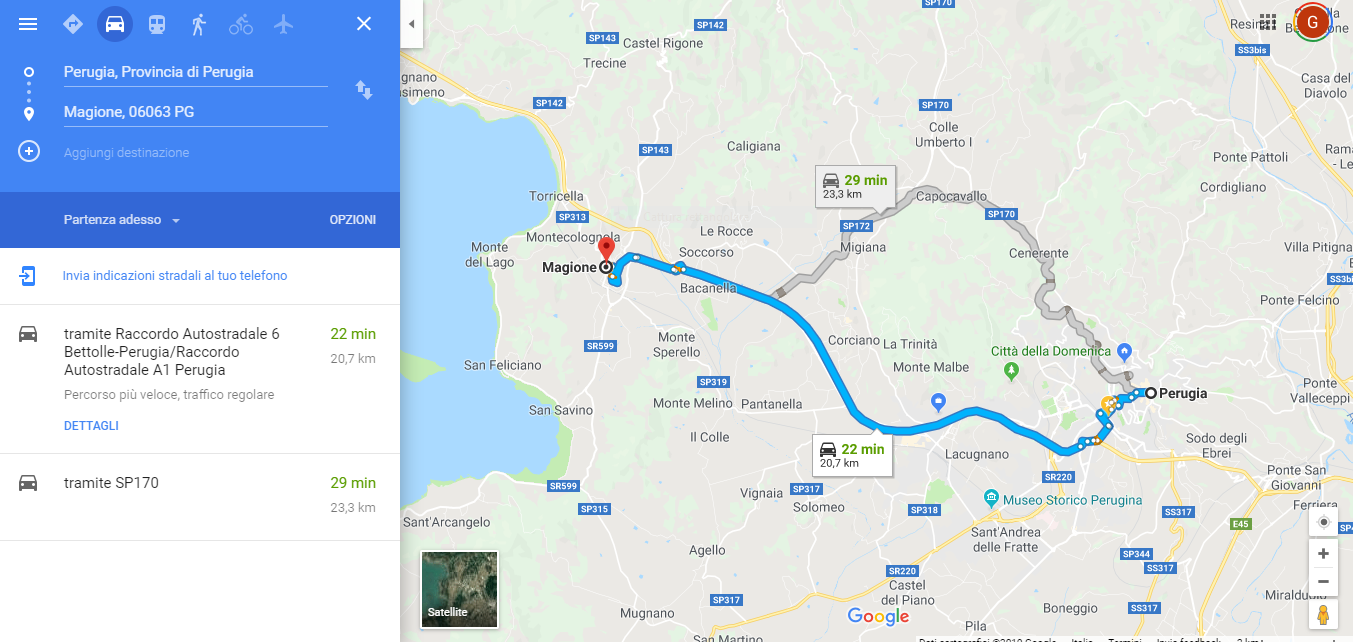
\includegraphics[width=0.9\linewidth]{directionMode}
\end{center}
 (ETA:Estimated Time of Arrival). È  questo il termine esteso dell’acronimo più utilizzato nel settore della navigazione satellitare, e che abbiamo imparato a conoscere meglio con l’evolversi della tecnologia e del software a bordo dei nostri dispositivi. ETA significa quindi “tempo stimato per l’arrivo a destinazione“, e naturalmente fornisce semplicemente una “stima” o una “previsione” di quanto lungo può essere un viaggio a seconda del percorso e del mezzo che scegliamo.
Come in altri prodotti simili, gli ETA di Google Maps sono basati su una varietà di cose, a seconda dei dati che sono disponibili in una particolare area. Queste cose vanno dai limiti di velocità ufficiali a quelli raccomandati, come la velocità calcolata a seconda del tipo di strada, i dati della media storica su un certo periodo di tempo (a volte solo media, a volte in particolari momenti del giorno), il reale tempo di viaggio di utenti precedenti ed informazioni sul traffico in tempo reale. Alla fine si sovrappongono i dati provenienti da tutte queste fonti e viene fornita la migliore approssimazione possibile. È dunque questo il “segreto” del calcolo degli ETA di Google Maps, cioè mixare una serie di dati provenienti da più fonti per ricavare un tempo stimato di percorrenza il più preciso possibile.\\
Anche se ormai si è raggiunto un livello molto alto di previsione del tempo di arrivo, c’è sempre da considerare un’incertezza intrinseca che fa si che gli ETA risultino sempre non precisissimi, ed il motivo è il seguente:\\
Calcolare gli ETA è un problema di previsione del futuro, ed il traffico che segue determinati schemi è intrinsecamente imprevedibile. Anche se hai la completa conoscenza delle condizioni correnti del traffico e conosci le variazioni del percorso (ad esempio l’inizio di lavori o la fine di una partita di football), non c’è niente che può prevedere un incidente o un camion che procede lentamente per cambiare itinerario.
\subsubsection{Street View mode}
Maps Embed API consente di visualizzare le immagini Street View come panorami interattivi. Google Street View fornisce viste panoramiche da posizioni designate in tutta la sua area di copertura. Sono inoltre disponibili collezioni speciali Street View.\\
\begin{center}
	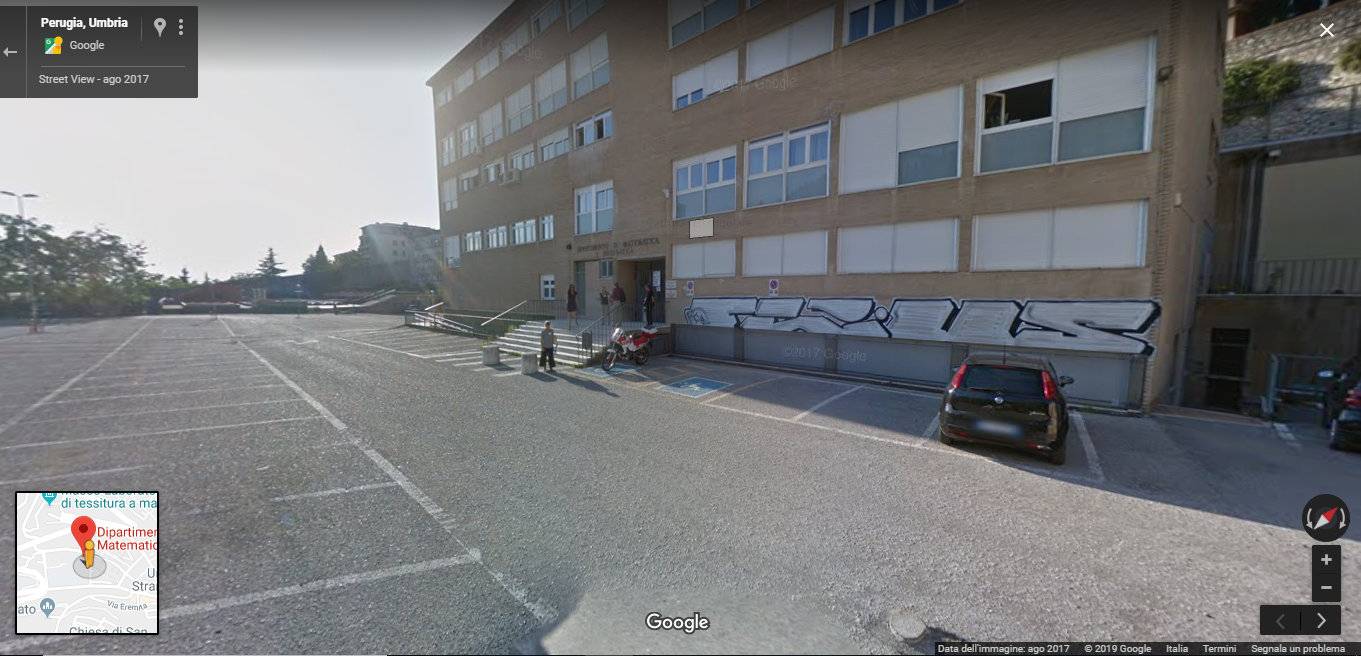
\includegraphics[width=0.9\linewidth]{dipartStreetView}
\end{center}
Ogni panorama di Street View offre una vista completa a 360 gradi da un'unica posizione. Le immagini contengono una vista orizzontale a 360 gradi (una vista panoramica completa) e verticale a 180 gradi (da dritto verso l'alto a dritto verso il basso). La modalità streetview fornisce uno spettatore che rende il panorama risultante come una sfera con una telecamera al centro. È possibile manipolare la fotocamera per controllare lo zoom e l'orientamento della fotocamera.
\subsubsection{Search mode}
La modalità di ricerca visualizza i risultati di una ricerca nella regione della mappa visibile sul dispositivo.
\subsection{DirectionService (Calcolare la direzione e il tempo dello spostamento)}
È possibile calcolare le indicazioni stradali (utilizzando diversi metodi di trasporto) utilizzando l'oggetto DirectionService. Questo oggetto comunica con l'API Directions Service di Google Maps che riceve le richieste di direzione e restituisce un percorso efficiente. Il tempo di percorrenza è il fattore primario che viene ottimizzato prendendo in considerazione parametri precedentemente descritti.
\subsubsection{Gestire le richieste di direzione}
L'accesso al servizio Directions è asincrono, in quanto l'API di Google Maps deve effettuare una chiamata ad un server esterno. Per questo motivo, è necessario passare un metodo di callback da eseguire al termine della richiesta. Questo metodo di callback dovrebbe elaborare i risultati inviati.
\textit{\textbf{Come fa? ... }}\\
Per utilizzare le direzioni nelle API JavaScript delle mappe, creare un oggetto di tipo DirectionsService e chiamare DirectionsService.route() per avviare una richiesta al servizio Directions, passandogli un oggetto DirectionsRequest letteralmente contenente i termini di input e un metodo di callback da eseguire al ricevimento della risposta.
L'oggetto DirectionsRequest letteralmente contiene i seguenti campi:
\lstset{frameround=fttt}
\begin{lstlisting}[frame=trBL]
{
origin: LatLng | String | google.maps.Place,
destination: LatLng | String | google.maps.Place,
travelMode: TravelMode,
transitOptions: TransitOptions,
drivingOptions: DrivingOptions,
unitSystem: UnitSystem,
waypoints[]: DirectionsWaypoint,
optimizeWaypoints: Boolean,
provideRouteAlternatives: Boolean,
avoidFerries: Boolean,
avoidHighways: Boolean,
avoidTolls: Boolean,
region: String
}
\end{lstlisting}
Spiegazione dei campi:
\begin{itemize}
	\item \textbf{origin: }Deve essere messo obbligatoriamente in quanto specifica il punto di partenza del nostro percorso. Questo valore può essere specificato come stringa (per esempio, "Perugia, IT"), come valore LatLng o come oggetto google.maps.place. Se si utilizza un oggetto google.maps.maps.Place, è possibile specificare un ID luogo, una stringa di interrogazione o una posizione LatLng. È possibile recuperare gli ID dei luoghi dai servizi Geocoding, Place Search e Place Autocomplete nelle API JavaScript Maps.
	\item \textbf{destination: }Anch'esso deve essere obbligatoriamente presente, specifica il punto finale verso il quale calcolare le direzioni. Le opzioni sono le stesse del campo origine descritto sopra.
	\item \textbf{travelMode: }(Obbligatorio) Specifica la modalità di trasporto da utilizzare per il calcolo delle direzioni.\\I valori validi sono specificati nelle seguenti modalità di trasporto:
	\subitem{\textbf{Auto:} }Indica le direzioni di guida standard utilizzando la rete stradale.
	\subitem{\textbf{Moto:} }indica le direzioni di guida in moto utilizzando la rete stradale.
	\subitem{\textbf{Mezzi pubblici:} }Indicazioni stradali attraverso le vie di trasporto pubblico.
	\subitem{\textbf{A piedi:} }Indicazioni stradali attraverso sentieri pedonali e marciapiedi.
	\item {\textbf{transitOptions: (Opzionale)} }Le opzioni di transito disponibili  variano a seconda delle modalità di viaggio. 
	 \begin{lstlisting}[frame=trBL]
	{
	arrivalTime: Date,
	departureTime: Date,
	modes[]: TransitMode,
	routingPreference: TransitRoutePreference
	}
	\end{lstlisting}
	L'oggetto TransitOptions contiene letteralmente i seguenti campi(opzionali):\\
		Nel caso di un trasporto pubblico è possibile specificare nel campo (\textit{arrival/departure Time}) orario della partenza e tipo( \textit{modes[ ]}) di trasporto scelto: pullman o treno etc.
    \subsubitem {\textbf{RoutingPreference(Preferenze di percorso):} } (opzionale) Specifica le preferenze per le vie di transito. Usando questa opzione, si possono influenzare le opzioni restituite ossia si può scegliere quale percorso seguire, piuttosto che accettare la migliore rotta predefinita scelta dall'API. Questo campo può essere specificato solo se la richiesta include una chiave API. Possiamo impostare la soluzione indicando dei limiti nelle modalità di "cambio" di mezzi di trasporto o nello spostamento a piedi:
   \subsubitem FEWER TRANSFERS indica che il percorso calcolato dovrebbe preferire un numero limitato di trasferimenti.
    \subsubitem LESS WALKING indica che il percorso calcolato dovrebbe preferire quantità limitate di spostamenti a piedi.

Un esempio di algoritmo per definire le opzioni di trasferimento può essere scritto così:
\begin{lstlisting}[frame=trBL]
{
origin: 'Perugia,IT',
destination: 'Magione,IT',
travelMode: 'TRANSIT', //transit sta per "mezzi pubblici"
transitOptions: {
departureTime: new Date(dataDiPartenza),
modes: ['BUS'],
routingPreference: 'FEWER_TRANSFERS'},
unitSystem: google.maps.UnitSystem.IMPERIAL
}
\end{lstlisting} 

\item{\textbf{DrivingOption:} }(opzionale) specifica valori che si applicano solo alle richieste in cui travelMode è DRIVING (Auto). \\ \textbf{Al suo interno è possibile scegliere il tragitto con o senza traffico e tutte le opzioni attraverso le quali l'app riesce a stabilire il tempo di percorrenza da un origine ad una destinazione indicate}
Si può stabilire la soluzione ottima, la peggio o una intermedia, in base all'opzione scelta vengono fatte diverse considerazioni per l'algoritmo da seguire nel restituire il tempo di percorrenza richiesto. Esempio se si sceglie l'opzione "ottima" verranno applicate le modalità di percorrenza dettate attraverso un algoritmo dal mix di esperienza di chi ha condotto quelle tratte e dalle statistiche del traffico in base alle ore della giornata. Di seguito riporto un esempio:
\begin{lstlisting}[frame=trBl]
drivingOptions: {
departureTime: new Date(Date.now() + N),
trafficModel: 'optimistic' //scelta ottima 
}
\end{lstlisting}
\item \textbf{UnitSystem: (opzionale)} specifica quale unità di sistema utilizzare per la visualizzazione dei risultati.
\item \textbf{waypoints[ ]: (opzionale}) Specifica un array di DirectionsWaypoints. I waypoint modificano una rotta instradandola attraverso le posizioni specificate. E' utile quando non scegliamo il percorso di default ma uno voluto da noi.  
\end{itemize}



\section{Metodi di tracciamento (Google Maps)}
Supponendo di avere le api di google maps a disposizione, come possiamo dunque stabilire come fa un applicazione mobile a capire se ci muoviamo in moto in macchina o a piedi in un tragitto da origine a destinazione? ... 
Considerando le informazioni date dalle api di google e assumendo che attraverso statistiche e informazioni riguardanti il traffico a seconda dell'orario di percorrenza si può fare una distinzione tra macchina e moto tenendo conto che con la moto si può destreggiare meglio nel traffico, evitando eventuali lunghe code nelle quali in macchina si è costretti ad aspettare lo sgombro del traffico. E impostando il percorso, questo è possibile attraverso GPS saperlo prima. Viste le diverse dimensioni dei mezzi si può anche pensare ad eventuali scorciatoie di tragitto in cui si può passare solo in moto o comunque non certamente con la macchina. In questo modo tenendo conto anche della cronologia delle posizioni si può evidenziare una differenza nel fare lo stesso percorso (in luoghi agibili con mezzi ridotti all'auto) ad esempio di corsa o in bicicletta, perchè in moto si andrebbe in ogni caso più veloce. A parità di "spazi" si può tenere conto delle inclinazioni del dispositivo nel caso in cui si affrontino molte curve, ovviamente queste considerazioni vanno fatte tenendo presente il tempo di arrivo. Se muovessi il telefono inclinandolo mentre cammino o mentre sono in auto salvo in caso di percorsi privi di curve si può cmq stabilire una differenza di percorrenza in moto o in auto o a piedi. Un idea potrebbe essere anche impostare nel dispositivo dei sensori per percepire il forte "rumore" o le vibrazioni che comportano il viaggio in moto, un auto specialmente quelle degli ultimi tempi non è paragonabile in questi termini ad una moto, così da percepire una anche lieve differenza.





\end{document}
